\documentclass[12pt,aspectratio=43,dvipsnames,table]{beamer}
\usepackage[french]{babel}
\usepackage[T1]{fontenc}
\usepackage[utf8]{inputenc}
\usepackage{url}
\usepackage{multirow}
% \usepackage{euler}
% \usepackage{color}

\usetheme{default}
\useinnertheme{default}
\useoutertheme{default}
\usefonttheme{serif}
\usecolortheme[named=WildStrawberry]{structure}

% Marges autour des slides
\setbeamersize{text margin left=5mm, text margin right=5mm}

% Suppression des symboles de navigation
\beamertemplatenavigationsymbolsempty

% Définition du pied de page
\setbeamertemplate{footline} {
  \hfill{
    \insertshortdate ~- %
    page \insertframenumber~sur~\inserttotalframenumber %
    %\hspace*{0.1cm}
  } \vspace*{0.05cm}
}

% Définition des espacements des listes
\setlength{\leftmargini}{0.6cm}
\setlength{\leftmarginii}{0.4cm}
\setlength{\leftmarginiii}{0.4cm}

\title{Recherche d'information cross-lingue}
\subtitle{Applications multilingues - module X9IT100}
\author{Florian Boudin}
\institute{Département informatique, Université de Nantes}
\date[30 juillet 2013 / Rév.~1]{Révision~1 du 30 juillet 2012}

\begin{document}


%-B--------------------------------------------------------------------------B-%
\frame[plain]{\titlepage}
%-E--------------------------------------------------------------------------E-%


%##############################################################################%
\section{Introduction}
%##############################################################################%


%-B--------------------------------------------------------------------------B-%
\begin{frame}
    \frametitle{Préface}
    \begin{itemize} \itemsep10pt
        \item Volume horaire (2h40)
        \item Notions abordées dans ce cours
        \begin{itemize}
            \item Recherche d'Information (rappels)
            \item 
        \end{itemize}
        \item Ce cours est basé sur le livre \textit{Cross-Language Information 
              Retrieval} de Jian-Yun Nie~\cite{DBLP:series/synthesis/2010Nie}.
    \end{itemize}
\end{frame}
%-E--------------------------------------------------------------------------E-%


%-B--------------------------------------------------------------------------B-%
\begin{frame}
    \frametitle{Introduction}
    \begin{itemize} \itemsep10pt
        \item La \textbf{Recherche d'Information} (RI) fait partie intégrante de
              notre vie quotidienne.
        \item Dans la plupart des cas, nous recherchons des documents rédigés 
              dans notre langue maternelle, en général celle utilisée dans la 
              requête.
        \item \textbf{Cependant...}
        \begin{itemize}
            \item L'information pertinente n'est pas toujours disponible dans 
                  notre langue maternelle.
            \item Le web offre une mine d'information riche et multilingue à 
                  laquelle nous souhaitons avoir accès.
        \end{itemize}
        \item \'Emergence de la problématique de la RI cross-lingue
    \end{itemize}
\end{frame}
%-E--------------------------------------------------------------------------E-%


%##############################################################################%
\section{Recherche d'information (rappels)}
%##############################################################################%


%-B------------------------------PLAN----------------------------------------B-%
\begin{frame}
\frametitle{Plan}
\tableofcontents[sectionstyle=show,subsectionstyle=hide,subsubsectionstyle=hide]
\end{frame}
%-E--------------------------------------------------------------------------E-%


%-B--------------------------------------------------------------------------B-%
\begin{frame}
    \frametitle{Le processus de recherche d'information}
    \begin{figure}
    \centering
    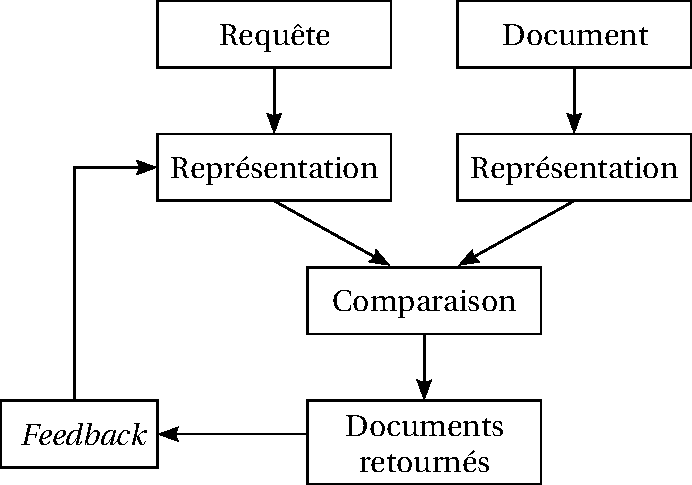
\includegraphics[width=0.75\textwidth]{img/typicalIR.pdf}
    \caption{Processus de recherche d'information (Figure 1.1 
             de~\cite{DBLP:series/synthesis/2010Nie}).}
    \end{figure}
\end{frame}
%-E--------------------------------------------------------------------------E-%


%-B--------------------------------------------------------------------------B-%
\begin{frame}
    \frametitle{Modèles de RI}
    \begin{itemize} \itemsep10pt
        \item Un modèle définit la représentation des documents et des requêtes 
              ainsi que la fonction de pondération.
        \item La plupart des modèles sont construits sur la notion de 
              \textit{terme}, qui peut être un mot (e.g.~\textit{computer}), un 
              stem (e.g.~\textit{comput}) ou une expression multimots 
              (e.g.~\textit{computer system}).
        \item Modèles de RI classiques
        \begin{itemize}
            \item Modèle booléen
            \item Modèle vectoriel, i.a.~\cite{DBLP:journals/cacm/SaltonWY75}
            \item Modèle probabiliste, i.a.~\cite{robertson1976relevance}
            \item Modèle de langue, i.a.~\cite{DBLP:conf/sigir/PonteC98}
        \end{itemize}
    \end{itemize}
\end{frame}
%-E--------------------------------------------------------------------------E-%


%-B--------------------------------------------------------------------------B-%
\begin{frame}[allowframebreaks]
    \frametitle{\'Evaluation}
    \begin{itemize} \itemsep10pt
        \item Plusieurs mesures ont été proposées pour évaluer l'efficacité des
              systèmes de RI.
        \item Les mesures de base sont la précision et le rappel.
    \end{itemize}

    \begin{equation}
      \text{precision} = \frac{\text{\# documents pertinents retrouvés}}
                              {\text{\# documents retrouvés}}
    \end{equation}

    \begin{equation}
      \text{rappel} = \frac{\text{\# documents pertinents retrouvés}}
                           {\text{\# documents pertinents dans la collection}}
    \end{equation}

    \framebreak

    \begin{itemize} \itemsep10pt
        \item Une autre mesure largement utilisée est la \textit{Mean Average 
              Precision} (MAP)
    \end{itemize}

    \begin{equation}
      \text{MAP} = \frac{1}{M} \sum_{j=1}^{M} \Bigg( 
                     \frac{1}{N_j} \sum_{i=1}^{N_j} pr(d_{ij})
                   \Bigg)
    \end{equation}

    \begin{equation}
      pr(d_{ij}) = \left\{ 
        \begin{array}{l l}
          \frac{r_{ni}}{n_i} & \quad \text{si $n_i <$ MAX}\\
          0 & \quad \text{autrement}
        \end{array} \right.
    \end{equation}



\end{frame}
%-E--------------------------------------------------------------------------E-%


%##############################################################################%
\section{Les problèmes de langue en RI}
%##############################################################################%


%-B------------------------------PLAN----------------------------------------B-%
\begin{frame}
\frametitle{Plan}
\tableofcontents[sectionstyle=show,subsectionstyle=hide,subsubsectionstyle=hide]
\end{frame}
%-E--------------------------------------------------------------------------E-%


%-B--------------------------------------------------------------------------B-%
\begin{frame}
    \frametitle{}
\end{frame}
%-E--------------------------------------------------------------------------E-%


%-B--------------------------------------------------------------------------B-%
\begin{frame}
    \frametitle{}
\end{frame}
%-E--------------------------------------------------------------------------E-%


%##############################################################################%
\section{Références}
%##############################################################################%


%-B--------------------------------------------------------------------------B-%
\begin{frame}
    \frametitle{References}
    \bibliographystyle{alpha}
    \bibliography{bibliography}
\end{frame}
%-E--------------------------------------------------------------------------E-%


\end{document}